\section{Overview}

These appendices describe interfaces for a software package written in Python whose intent is to model the micro-mechanical response of alveolar sacs that comprise the bulk of the parenchyma in lung tissue.  A flow chart for this software is presented in Fig.~\ref{figFlow}.  The software assumes the following design strategy: \textit{i\/}) a reference configuration exists (see \P\ below) and three sequential configurations exist that are separated in time by an uniform time step, \textit{ii\/}) the three sequential configurations associate with steps $n \! - \! 1$, $n$ and $n \! + \! 1$, \textit{iii\/}) co-ordinates for the next configuration are assigned through a vertex's \texttt{update} method (they can be reassigned multiple times at any step along a solution path), \textit{iv\/}) the \texttt{advance} method relabels the current data to their associated previous data, and then relabels the next data to their associated current data, thereby preparing the data structure of each object within a dodecahedral object for its next step along a solution path, and \textit{v\/}) the mechanical response is isotropic and can be described by three modes of deformation: dilatation\slash dilation, squeeze and shear \cite{Freedetal17,FreedZamani19}.

\begin{sidewaysfigure}
	\centering
	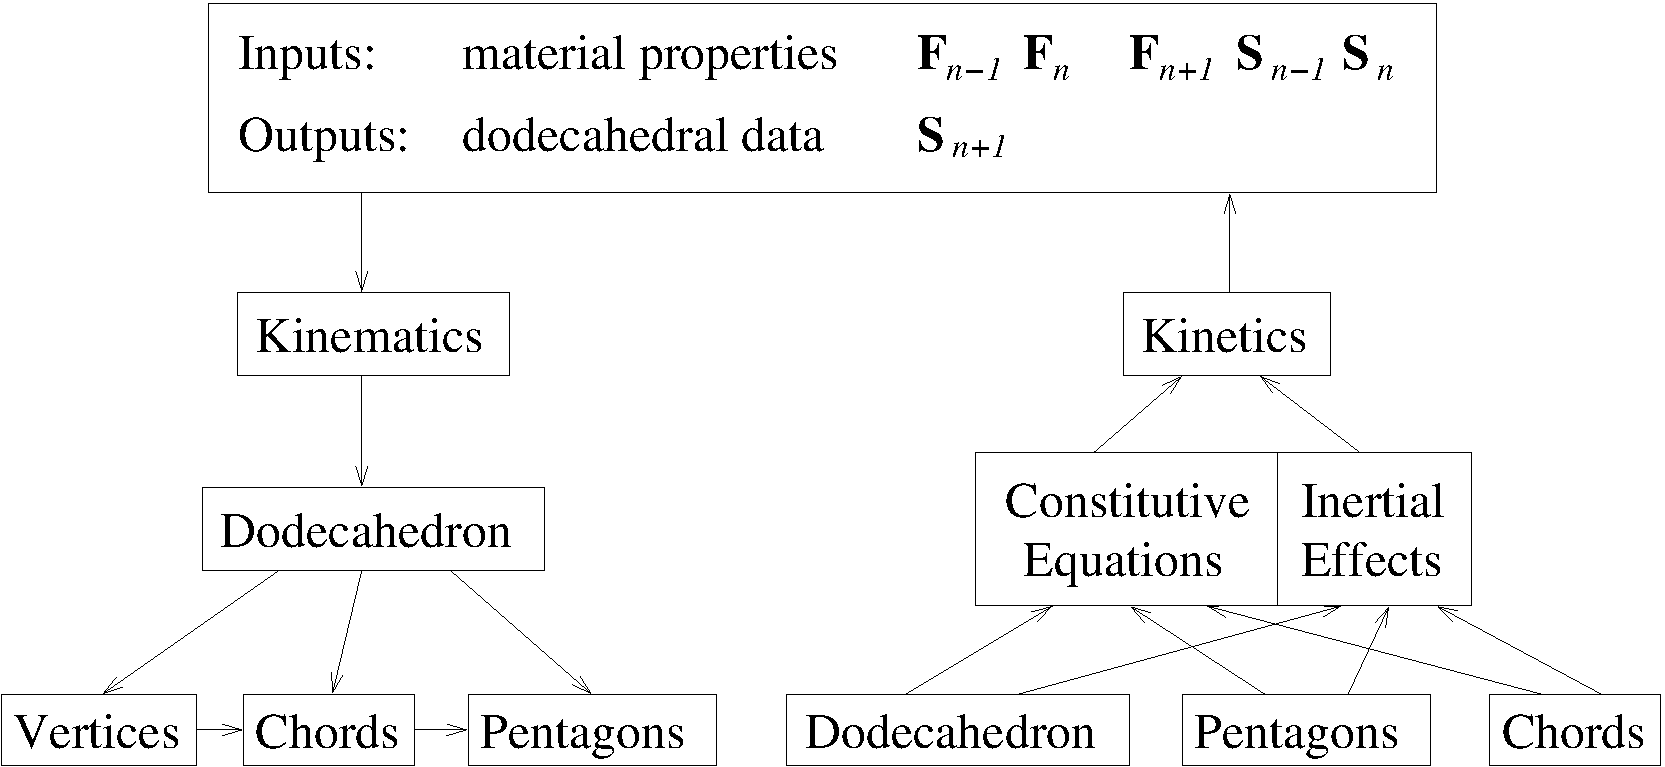
\includegraphics[width=\columnwidth]{figures/flow.pdf}
	\caption{Flow chart for a dodecahedral model of an alveolus.}
	\label{figFlow}
\end{sidewaysfigure}

The initial co-ordinates that locate each vertex in a dodecahedron used to model the alveoli of lung are assigned according to a reference configuration where the pleural pressure (the negative pressure surrounding lung in the pleural cavity) and the transpulmonary pressure (the difference between aleolar and pleural pressures) are both at zero gauge pressure, i.e., \textit{all pressures are atmospheric pressure in the reference state.}  This is not a typical physiological state.  The pleural pressure is normally negative, sucking the pleural membrane against the wall of the chest.  During expiration, the diaphragm is pushed up, reducing the pleural pressure.  The pleural pressure remains negative during breating at rest, but it can become positive during active expiration.  The surface tension created by surfactant helps keep most alveoli open during excursions into positive pleural pressures, but not all will remain open. Alveolar recruitment is not addressed here.  Under normal conditions, alveoli are their smallest at max expiration.  Alveolar size is predominately determined by the transpulmonary pressure.  The greater the transpulmonary pressure the greater the alveolar size.

Numerous methods belonging to the classes of these appendices have a string argument that is denoted as \texttt{state}  which can take on any of the following values:
\begin{labeling}{`p', `prev', `previous'}
\item [`c', `curr', `current'] gets the value for a current configuration 
\item [`n', `next'] gets the value for a next configuration 
\item [`p', `prev', `previous'] gets the value for a previous configuration 
\item [`r', `ref', `reference'] gets the value for the reference configuration 
\end{labeling}
Several strings can be used to denote each \texttt{state}.
